\documentclass[aspectratio=169,11pt]{beamer}
\usepackage[T2A]{fontenc}
\usepackage[utf8]{inputenc}
\usepackage[russian]{babel}
\usepackage{graphicx}
\usepackage{listings}
\usetheme{Madrid}
\usecolortheme{seahorse}
\setbeamertemplate{navigation symbols}{}
\setbeamertemplate{footline}[frame number]
\definecolor{codebg}{RGB}{246,247,249}
\lstset{
  language=Python,
  basicstyle=\ttfamily\fontsize{9}{11}\selectfont,
  keywordstyle=\color{blue!65!black},
  commentstyle=\color{green!40!black},
  stringstyle=\color{orange!60!black},
  backgroundcolor=\color{codebg},
  showstringspaces=false,
  columns=fullflexible,
  keepspaces=true,
  breaklines=true,
  frame=single,
  literate={А}{{\CYRA}}1 {Б}{{\CYRB}}1 {В}{{\CYRV}}1 {Г}{{\CYRG}}1
           {Д}{{\CYRD}}1 {Е}{{\CYRE}}1 {Ё}{{\CYRYO}}1 {Ж}{{\CYRZH}}1
           {З}{{\CYRZ}}1 {И}{{\CYRI}}1 {Й}{{\CYRISHRT}}1 {К}{{\CYRK}}1
           {Л}{{\CYRL}}1 {М}{{\CYRM}}1 {Н}{{\CYRN}}1 {О}{{\CYRO}}1
           {П}{{\CYRP}}1 {Р}{{\CYRR}}1 {С}{{\CYRS}}1 {Т}{{\CYRT}}1
           {У}{{\CYRU}}1 {Ф}{{\CYRF}}1 {Х}{{\CYRH}}1 {Ц}{{\CYRC}}1
           {Ч}{{\CYRCH}}1 {Ш}{{\CYRSH}}1 {Щ}{{\CYRSHCH}}1 {Ъ}{{\CYRHRDSN}}1
           {Ы}{{\CYRERY}}1 {Ь}{{\CYRSFTSN}}1 {Э}{{\CYREREV}}1 {Ю}{{\CYRYU}}1
           {Я}{{\CYRYA}}1 {а}{{\cyra}}1 {б}{{\cyrb}}1 {в}{{\cyrv}}1
           {г}{{\cyrg}}1 {д}{{\cyrd}}1 {е}{{\cyre}}1 {ё}{{\cyryo}}1
           {ж}{{\cyrzh}}1 {з}{{\cyrz}}1 {и}{{\cyri}}1 {й}{{\cyrishrt}}1
           {к}{{\cyrk}}1 {л}{{\cyrl}}1 {м}{{\cyrm}}1 {н}{{\cyrn}}1
           {о}{{\cyro}}1 {п}{{\cyrp}}1 {р}{{\cyrr}}1 {с}{{\cyrs}}1
           {т}{{\cyrt}}1 {у}{{\cyru}}1 {ф}{{\cyrf}}1 {х}{{\cyrh}}1
           {ц}{{\cyrc}}1 {ч}{{\cyrch}}1 {ш}{{\cyrsh}}1 {щ}{{\cyrshch}}1
           {ъ}{{\cyrhrdsn}}1 {ы}{{\cyrery}}1 {ь}{{\cyrsftsn}}1 {э}{{\cyrerev}}1
           {ю}{{\cyryu}}1 {я}{{\cyrya}}1
           {°}{{\textdegree}}1 {²}{{\texttwosuperior}}1
}

\title{Графики и таблицы в Python}
\subtitle{Matplotlib, Seaborn и pandas: код и его результат}
\author{Школа 1514}
\date{Занятие 02}
\begin{document}
\begin{frame}\titlepage\end{frame}
\section{Matplotlib: начинаем с графика}
\begin{frame}{Matplotlib: начинаем с графика}
Matplotlib — библиотека Python для построения графиков. Она умеет рисовать линии, точки, столбцы и оси: нам не нужно программировать их отрисовку самим.
\medskip

Начнём с модуля pyplot. Его функции работают с текущим рисунком: построить, подписать, показать. Переменные fig и ax для первых примеров не нужны.
\medskip

На слайдах код находится слева, а справа — результат выполнения этого же кода. Примеры идут по порядку: созданные переменные используются дальше.
\end{frame}
% example:first-line
\begin{frame}[fragile]{Первый график: температура за неделю}
\begin{columns}[c,onlytextwidth]
\begin{column}{0.49\textwidth}
\begin{lstlisting}
import matplotlib.pyplot as plt

days = [1, 2, 3, 4, 5, 6, 7]
temperature = [15, 17, 16, 20, 19, 18, 21]
plt.plot(days, temperature)
plt.show()
\end{lstlisting}
\end{column}
\begin{column}{0.49\textwidth}
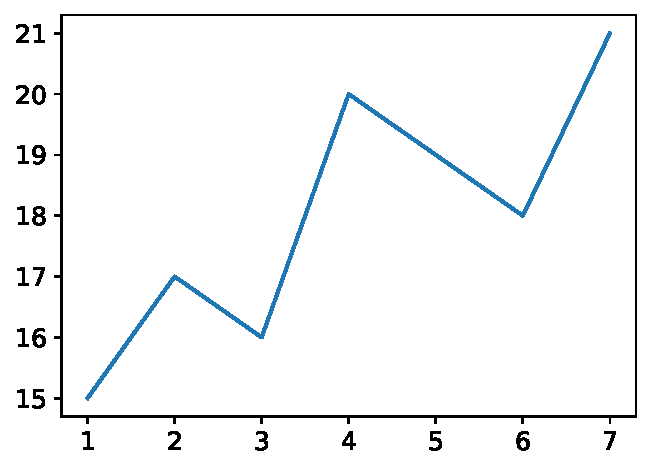
\includegraphics[width=\linewidth,height=0.59\textheight,keepaspectratio]{img/first-line.pdf}
\end{column}
\end{columns}
\medskip
\small Первый список задаёт x, второй — y. Видно, как температура менялась по дням; но без подписей посторонний читатель ещё не знает, что означают числа.
\end{frame}
% example:labels
\begin{frame}[fragile]{Добавляем смысл: оси, заголовок и точки}
\begin{columns}[c,onlytextwidth]
\begin{column}{0.49\textwidth}
\begin{lstlisting}
plt.plot(days, temperature, marker="o")
plt.xlabel("День")
plt.ylabel("Температура, °C")
plt.title("Температура за неделю")
plt.show()
\end{lstlisting}
\end{column}
\begin{column}{0.49\textwidth}
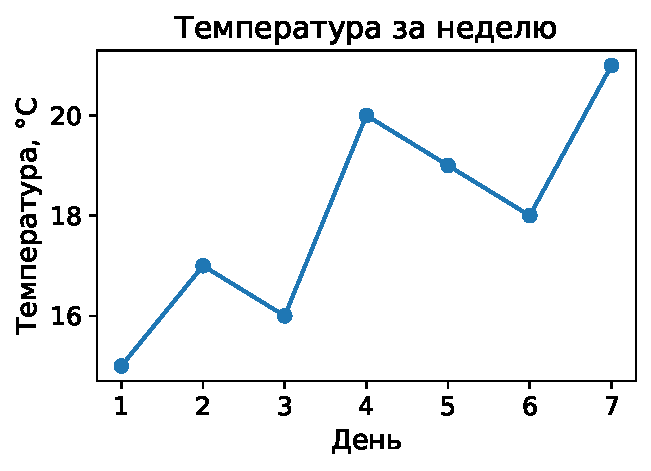
\includegraphics[width=\linewidth,height=0.59\textheight,keepaspectratio]{img/labels.pdf}
\end{column}
\end{columns}
\medskip
\small Кружки — измерения, линия помогает проследить изменение между соседними днями. Попробуйте заменить температуру седьмого дня на 16 и предскажите изменение графика.
\end{frame}
% example:two-lines
\begin{frame}[fragile]{Два города на одном рисунке}
\begin{columns}[c,onlytextwidth]
\begin{column}{0.49\textwidth}
\begin{lstlisting}
kazan = [13, 14, 17, 18, 16, 19, 20]
plt.plot(days, temperature,
         label="Москва")
plt.plot(days, kazan, label="Казань")
plt.xlabel("День")
plt.ylabel("Температура, °C")
plt.legend()
plt.show()
\end{lstlisting}
\end{column}
\begin{column}{0.49\textwidth}
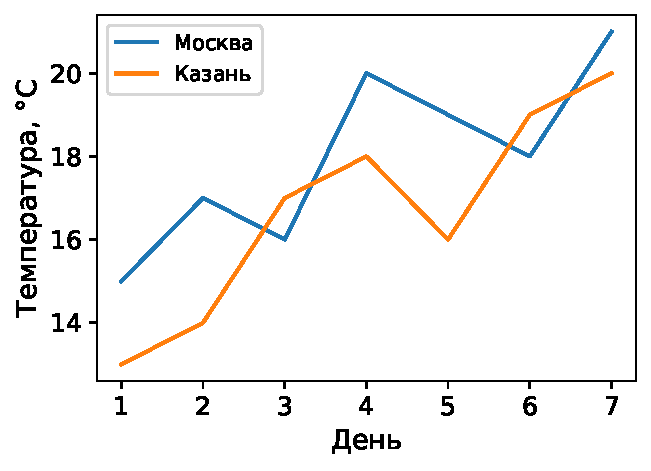
\includegraphics[width=\linewidth,height=0.59\textheight,keepaspectratio]{img/two-lines.pdf}
\end{column}
\end{columns}
\medskip
\small В четвёртый день в Москве 20 \ensuremath{^\circ}C, в Казани 18 \ensuremath{^\circ}C. Линии уместны: дни упорядочены, и соседство наблюдений имеет смысл.
\end{frame}
% example:function
\begin{frame}[fragile]{График математической функции}
\begin{columns}[c,onlytextwidth]
\begin{column}{0.49\textwidth}
\begin{lstlisting}
import numpy as np

x = np.linspace(-2, 2, 100)
plt.plot(x, x ** 2)
plt.xlabel("x")
plt.ylabel("y = x²")
plt.grid(True)
plt.show()
\end{lstlisting}
\end{column}
\begin{column}{0.49\textwidth}
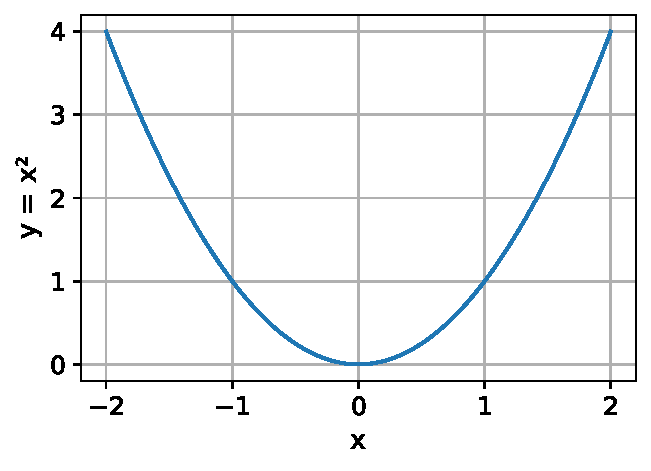
\includegraphics[width=\linewidth,height=0.59\textheight,keepaspectratio]{img/function.pdf}
\end{column}
\end{columns}
\medskip
\small Это та же команда plot, но данные не измерены, а вычислены. grid добавляет сетку. Попробуйте заменить x ** 2 на np.sin(x).
\end{frame}
% example:bike-scatter
\begin{frame}[fragile]{Scatter: расстояние и время поездки}
\begin{columns}[c,onlytextwidth]
\begin{column}{0.49\textwidth}
\begin{lstlisting}
distance = [2, 4, 6, 8, 10, 12]
minutes = [10, 18, 22, 35, 38, 48]
plt.scatter(distance, minutes)
plt.xlabel("Расстояние, км")
plt.ylabel("Время, мин")
plt.show()
\end{lstlisting}
\end{column}
\begin{column}{0.49\textwidth}
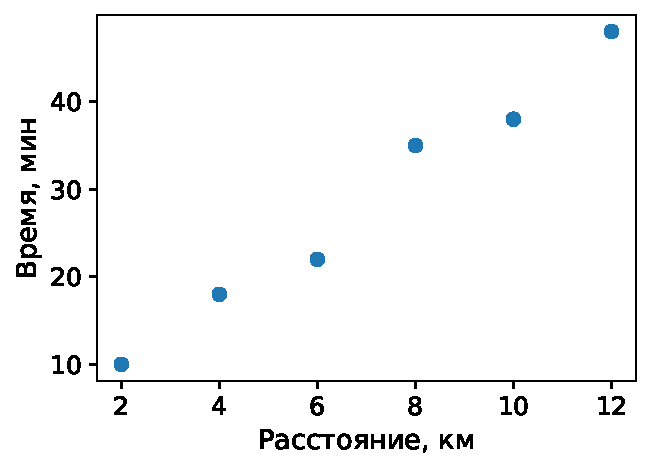
\includegraphics[width=\linewidth,height=0.59\textheight,keepaspectratio]{img/bike-scatter.pdf}
\end{column}
\end{columns}
\medskip
\small Большему расстоянию обычно соответствует большее время. Отдельные точки позволяют видеть отклонения, а не только общее направление связи.
\end{frame}
% example:cafe-bar
\begin{frame}[fragile]{Bar: сравниваем продажи напитков}
\begin{columns}[c,onlytextwidth]
\begin{column}{0.49\textwidth}
\begin{lstlisting}
drinks = ["Чай", "Кофе", "Какао"]
cups = [18, 32, 12]
plt.bar(drinks, cups)
plt.xlabel("Напиток")
plt.ylabel("Продано порций")
plt.show()
\end{lstlisting}
\end{column}
\begin{column}{0.49\textwidth}
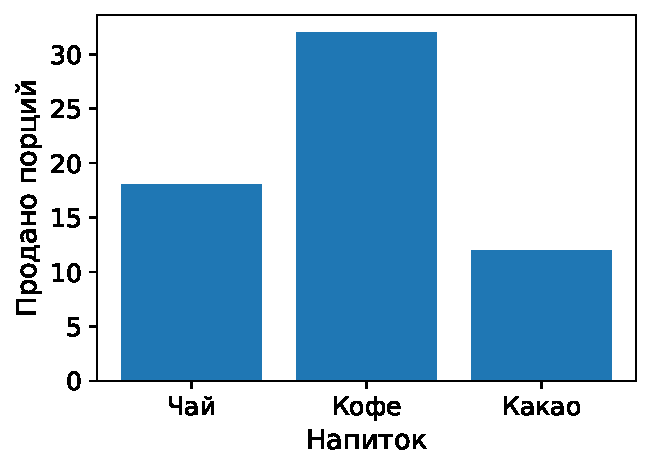
\includegraphics[width=\linewidth,height=0.59\textheight,keepaspectratio]{img/cafe-bar.pdf}
\end{column}
\end{columns}
\medskip
\small Кофе продали 32 порции, чая — 18. Столбцы подходят для категорий; соединять напитки линией обычно не имеет смысла.
\end{frame}
% example:wind-hist
\begin{frame}[fragile]{Hist: как распределена скорость ветра}
\begin{columns}[c,onlytextwidth]
\begin{column}{0.49\textwidth}
\begin{lstlisting}
wind = [1, 3, 2, 5, 4, 2, 6,
        3, 1, 4, 7, 5, 2, 3]
plt.hist(wind, bins=[0, 2, 4, 6, 8],
         edgecolor="white")
plt.xlabel("Скорость ветра, м/с")
plt.ylabel("Число измерений")
plt.show()
\end{lstlisting}
\end{column}
\begin{column}{0.49\textwidth}
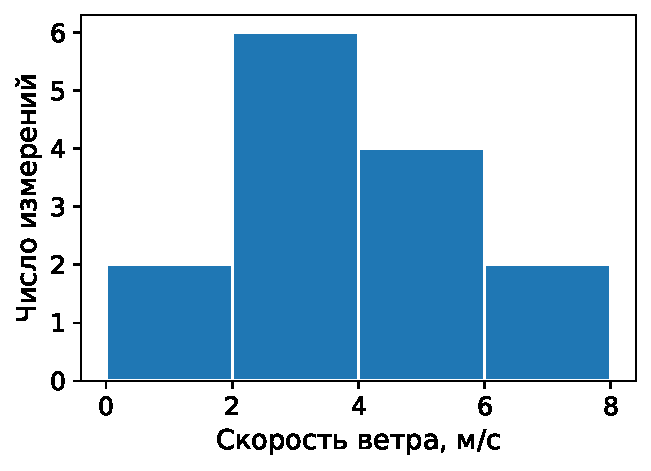
\includegraphics[width=\linewidth,height=0.59\textheight,keepaspectratio]{img/wind-hist.pdf}
\end{column}
\end{columns}
\medskip
\small В [2, 4) шесть измерений: три двойки и три тройки. Число 4 относится к [4, 6). Только последний интервал включает правую границу.
\end{frame}
\section{Pandas: зачем хранить данные в таблице}
\begin{frame}{Pandas: зачем хранить данные в таблице}
В кафе или магазине у каждой позиции есть название, категория, цена и число продаж. Если хранить всё отдельными списками, при сортировке легко потерять связь между товаром и его ценой. Таблица хранит эти значения вместе.
\medskip

pandas — библиотека Python для работы с таблицами. Она позволяет читать файлы, выбирать строки, считать по столбцам и получать сводки. Основной объект, DataFrame, — таблица с именованными столбцами. Начнём с четырёх товаров, чтобы каждый результат можно было проверить вручную.
\end{frame}
% example:create-table
\begin{frame}[fragile]{Создадим таблицу небольшого магазина}
\begin{columns}[c,onlytextwidth]
\begin{column}{0.49\textwidth}
\begin{lstlisting}
import pandas as pd

table = pd.DataFrame({
    "item": ["Тетрадь", "Блокнот",
             "Ручка", "Карандаш"],
    "category": ["Бумага", "Бумага",
                 "Письмо", "Письмо"],
    "price": [80, 120, 30, 20],
    "sold": [10, 5, 20, 15],
})
table
\end{lstlisting}
\end{column}
\begin{column}{0.49\textwidth}
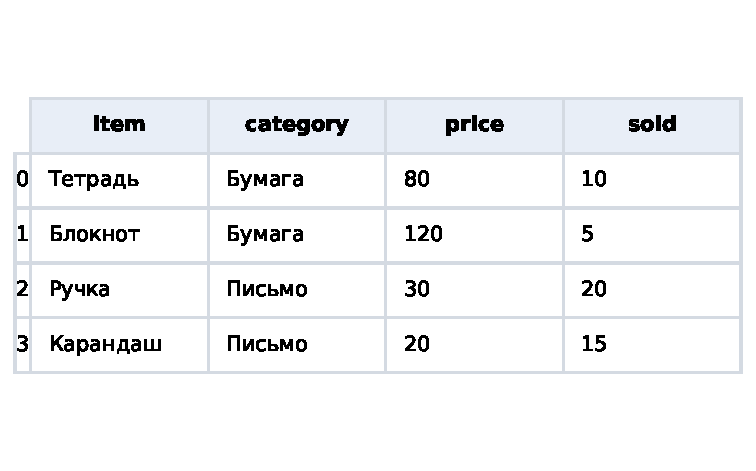
\includegraphics[width=\linewidth,height=0.59\textheight,keepaspectratio]{img/create-table.pdf}
\end{column}
\end{columns}
\medskip
\small pd — короткое имя pandas, ключи словаря стали названиями столбцов. Первая строка: тетрадь стоит 80 рублей, продано 10 штук. Числа 0–3 слева — индекс: метки строк, а не ещё один признак товара.
\end{frame}
% example:shape
\begin{frame}[fragile]{Размер таблицы и названия столбцов}
\begin{columns}[c,onlytextwidth]
\begin{column}{0.49\textwidth}
\begin{lstlisting}
print(table.shape)
print(len(table))
print(table.columns.tolist())
\end{lstlisting}
\end{column}
\begin{column}{0.49\textwidth}
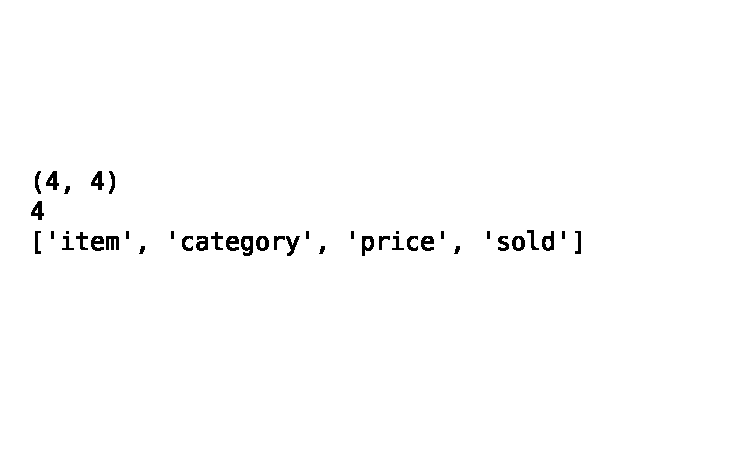
\includegraphics[width=\linewidth,height=0.59\textheight,keepaspectratio]{img/shape.pdf}
\end{column}
\end{columns}
\medskip
\small Получили четыре строки и четыре столбца. Эти команды только смотрят на таблицу и ничего из неё не удаляют.
\end{frame}
% example:series
\begin{frame}[fragile]{Выбираем один столбец}
\begin{columns}[c,onlytextwidth]
\begin{column}{0.49\textwidth}
\begin{lstlisting}
prices = table["price"]
prices
\end{lstlisting}
\end{column}
\begin{column}{0.49\textwidth}
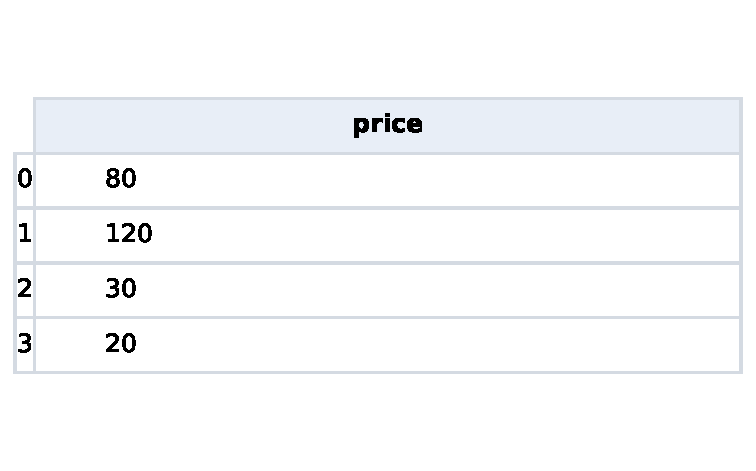
\includegraphics[width=\linewidth,height=0.59\textheight,keepaspectratio]{img/series.pdf}
\end{column}
\end{columns}
\medskip
\small Справа показаны индекс и значения выбранной Series. В Jupyter дополнительно появляется строка Name: price, dtype: int64 — имя столбца и тип его значений.
\end{frame}
% example:statistics
\begin{frame}[fragile]{Вычисляем по столбцу}
\begin{columns}[c,onlytextwidth]
\begin{column}{0.49\textwidth}
\begin{lstlisting}
print("Средняя цена:", prices.mean())
print("Минимум:", prices.min())
print("Максимум:", prices.max())
print("Всего продано:",
      table["sold"].sum())
\end{lstlisting}
\end{column}
\begin{column}{0.49\textwidth}
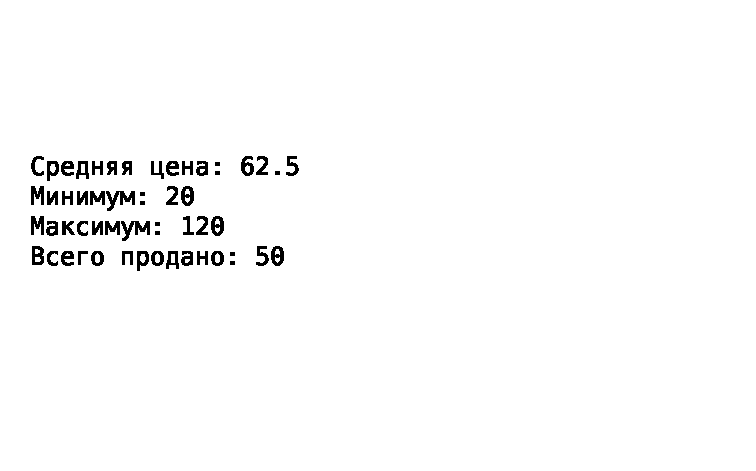
\includegraphics[width=\linewidth,height=0.59\textheight,keepaspectratio]{img/statistics.pdf}
\end{column}
\end{columns}
\medskip
\small Средняя цена: (80 + 120 + 30 + 20) / 4 = 62.5 рубля. Средняя цена товара здесь не взвешена по числу продаж.
\end{frame}
% example:columns
\begin{frame}[fragile]{Выбираем несколько столбцов}
\begin{columns}[c,onlytextwidth]
\begin{column}{0.49\textwidth}
\begin{lstlisting}
table[["item", "sold"]]
\end{lstlisting}
\end{column}
\begin{column}{0.49\textwidth}
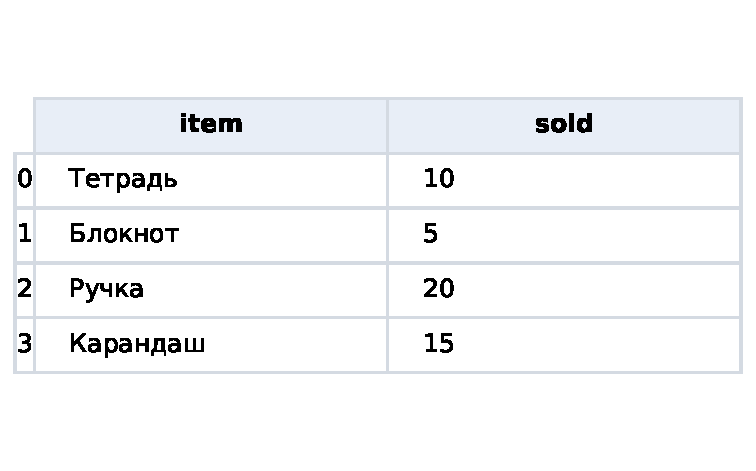
\includegraphics[width=\linewidth,height=0.59\textheight,keepaspectratio]{img/columns.pdf}
\end{column}
\end{columns}
\medskip
\small Теперь удобно смотреть только названия и количество продаж. Попробуйте вместо sold выбрать price и объяснить, что изменится.
\end{frame}
% example:mask
\begin{frame}[fragile]{Условие сначала даёт ответы True или False}
\begin{columns}[c,onlytextwidth]
\begin{column}{0.49\textwidth}
\begin{lstlisting}
mask = table["price"] >= 80
mask
\end{lstlisting}
\end{column}
\begin{column}{0.49\textwidth}
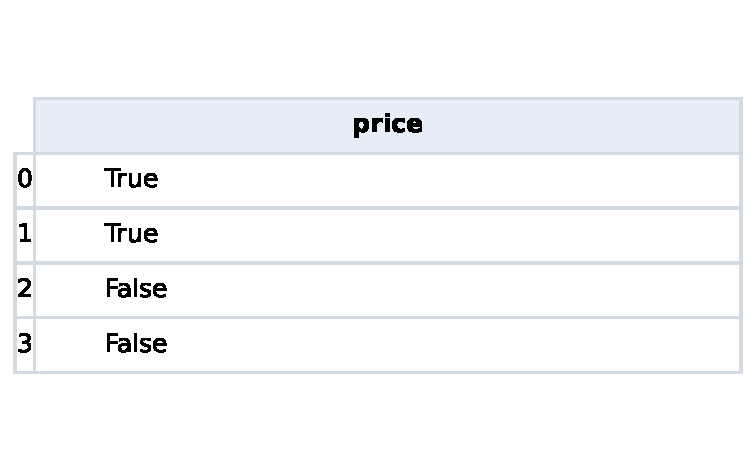
\includegraphics[width=\linewidth,height=0.59\textheight,keepaspectratio]{img/mask.pdf}
\end{column}
\end{columns}
\medskip
\small Тетрадь и блокнот подходят: напротив них True. Ручка и карандаш не подходят: напротив них False.
\end{frame}
% example:filter
\begin{frame}[fragile]{Используем маску для отбора строк}
\begin{columns}[c,onlytextwidth]
\begin{column}{0.49\textwidth}
\begin{lstlisting}
expensive = table[mask]
expensive
\end{lstlisting}
\end{column}
\begin{column}{0.49\textwidth}
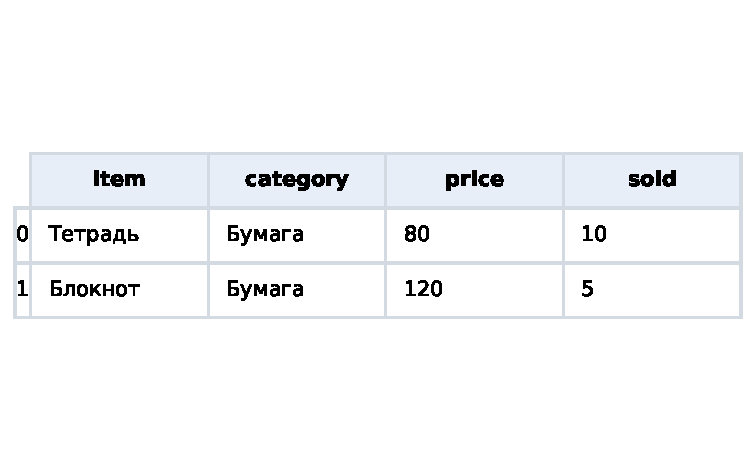
\includegraphics[width=\linewidth,height=0.59\textheight,keepaspectratio]{img/filter.pdf}
\end{column}
\end{columns}
\medskip
\small Остались два товара, а не два отдельных числа. Индексы сохранились из исходной таблицы. Попробуйте отобрать товары, которых продано больше 10 штук.
\end{frame}
% example:two-conditions
\begin{frame}[fragile]{Два условия одновременно}
\begin{columns}[c,onlytextwidth]
\begin{column}{0.49\textwidth}
\begin{lstlisting}
mask = ((table["category"] == "Письмо")
        & (table["sold"] >= 18))
table[mask]
\end{lstlisting}
\end{column}
\begin{column}{0.49\textwidth}
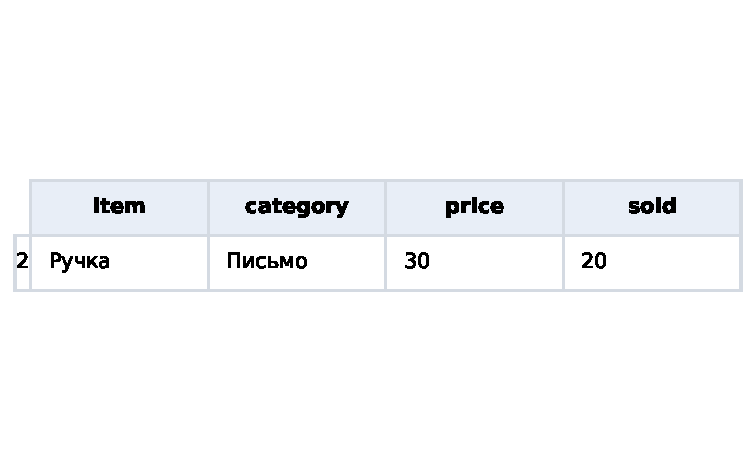
\includegraphics[width=\linewidth,height=0.59\textheight,keepaspectratio]{img/two-conditions.pdf}
\end{column}
\end{columns}
\medskip
\small В категории «Письмо» два товара, но не меньше 18 штук продано только ручек. Подходящая строка одна, и её индекс по-прежнему 2.
\end{frame}
% example:sort
\begin{frame}[fragile]{Упорядочим товары по продажам}
\begin{columns}[c,onlytextwidth]
\begin{column}{0.49\textwidth}
\begin{lstlisting}
popular = table.sort_values(
    "sold", ascending=False
)
popular
\end{lstlisting}
\end{column}
\begin{column}{0.49\textwidth}
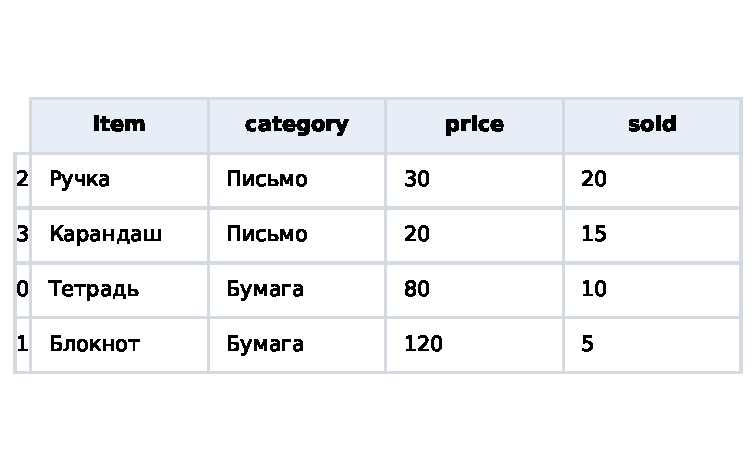
\includegraphics[width=\linewidth,height=0.59\textheight,keepaspectratio]{img/sort.pdf}
\end{column}
\end{columns}
\medskip
\small Первыми идут ручки: продано 20 штук. Исходная table не меняет порядок. popular.head(2) покажет два наиболее продаваемых товара.
\end{frame}
% example:revenue
\begin{frame}[fragile]{Новый столбец: выручка по каждому товару}
\begin{columns}[c,onlytextwidth]
\begin{column}{0.49\textwidth}
\begin{lstlisting}
table["revenue"] = (
    table["price"] * table["sold"]
)
table[["item", "revenue"]]
\end{lstlisting}
\end{column}
\begin{column}{0.49\textwidth}
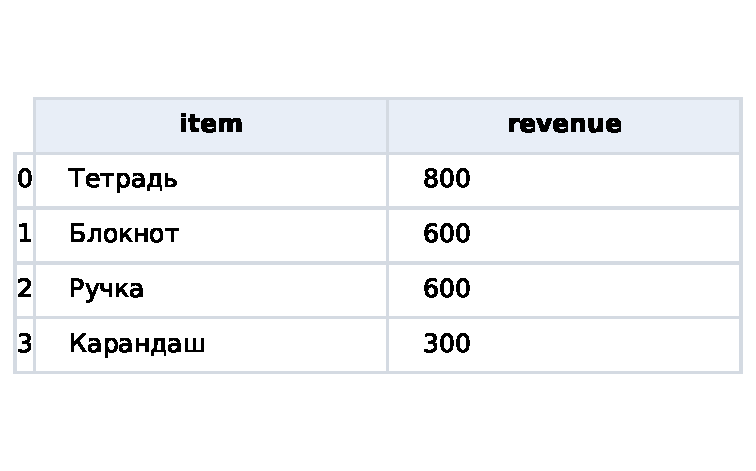
\includegraphics[width=\linewidth,height=0.59\textheight,keepaspectratio]{img/revenue.pdf}
\end{column}
\end{columns}
\medskip
\small Это выручка, не прибыль: расходы нам неизвестны. Справа для наглядности выведены только название и новый столбец.
\end{frame}
% example:groupby
\begin{frame}[fragile]{Groupby: отдельная сумма для каждой категории}
\begin{columns}[c,onlytextwidth]
\begin{column}{0.49\textwidth}
\begin{lstlisting}
groups = table.groupby("category")
revenue_by_category = (
    groups["revenue"].sum()
)
revenue_by_category
\end{lstlisting}
\end{column}
\begin{column}{0.49\textwidth}
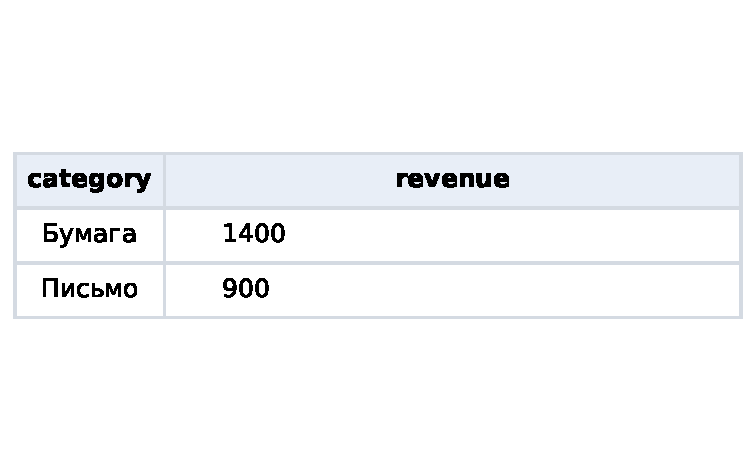
\includegraphics[width=\linewidth,height=0.59\textheight,keepaspectratio]{img/groupby.pdf}
\end{column}
\end{columns}
\medskip
\small В результате индекс — названия категорий, значения — их выручка. Получились 1400 и 900 рублей. Сам groupby ещё не считает: действие задаёт sum.
\end{frame}
% example:group-bar
\begin{frame}[fragile]{Покажем готовую сводку на графике}
\begin{columns}[c,onlytextwidth]
\begin{column}{0.49\textwidth}
\begin{lstlisting}
plt.bar(revenue_by_category.index,
        revenue_by_category.values)
plt.xlabel("Категория")
plt.ylabel("Выручка, руб.")
plt.show()
\end{lstlisting}
\end{column}
\begin{column}{0.49\textwidth}
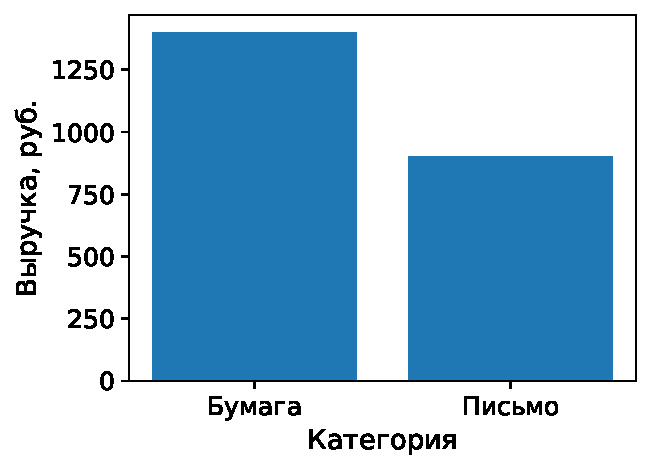
\includegraphics[width=\linewidth,height=0.59\textheight,keepaspectratio]{img/group-bar.pdf}
\end{column}
\end{columns}
\medskip
\small Высота столбца — выручка категории, а не количество товаров. Подпись оси y помогает не перепутать смысл агрегированных чисел.
\end{frame}
\section{Pandas: читаем данные о поездках}
\begin{frame}{Pandas: читаем данные о поездках}
Таблицу не обязательно создавать вручную. CSV — текстовый формат, где строки соответствуют наблюдениям, а значения разделены запятыми. Первая строка задаёт названия столбцов. read\_csv превращает такой файл в обычный DataFrame.
\medskip

В приложенном rides.csv одна строка — одна поездка на велосипеде. trip\_id — номер, bike — тип велосипеда, distance\_km — километры, minutes — время. Данные синтетические и не описывают реальных людей. После загрузки работают те же столбцы, маски и группировки, что и в маленьком примере магазина.
\end{frame}
% example:read-csv
\begin{frame}[fragile]{Загрузим файл и посмотрим начало}
\begin{columns}[c,onlytextwidth]
\begin{column}{0.49\textwidth}
\begin{lstlisting}
raw = pd.read_csv(DATA / "rides.csv")
raw.head(4)
\end{lstlisting}
\end{column}
\begin{column}{0.49\textwidth}
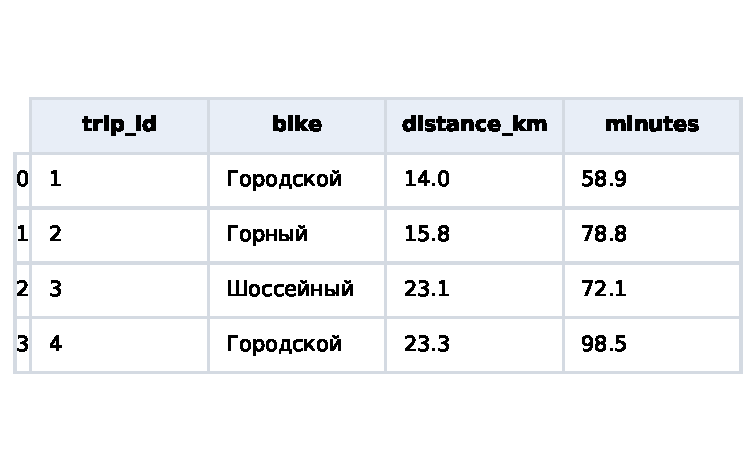
\includegraphics[width=\linewidth,height=0.59\textheight,keepaspectratio]{img/read-csv.pdf}
\end{column}
\end{columns}
\medskip
\small Одна поездка имеет и расстояние, и время, и тип велосипеда. Первые строки полезно прочитать словами перед тем, как считать статистики.
\end{frame}
% example:missing
\begin{frame}[fragile]{Размер и неизвестные значения}
\begin{columns}[c,onlytextwidth]
\begin{column}{0.49\textwidth}
\begin{lstlisting}
print("Размер:", raw.shape)
print("Пропуски:")
print(raw.isna().sum())
\end{lstlisting}
\end{column}
\begin{column}{0.49\textwidth}
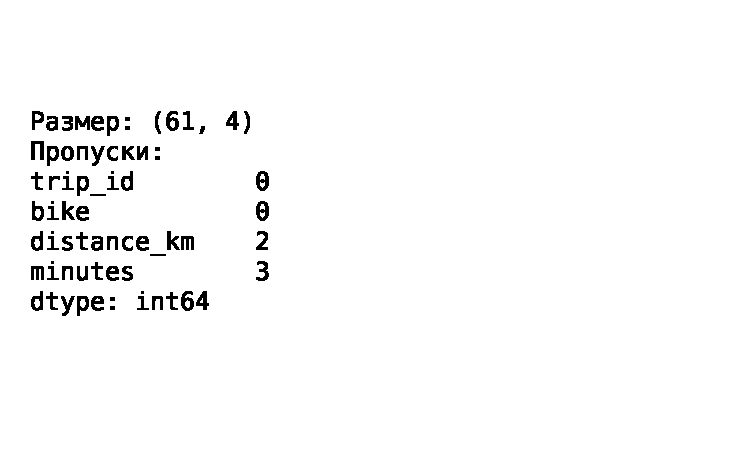
\includegraphics[width=\linewidth,height=0.59\textheight,keepaspectratio]{img/missing.pdf}
\end{column}
\end{columns}
\medskip
\small Всего 61 строка. Не записаны два расстояния и три длительности. Заменять их нулём означало бы придумать сведения, которых нет.
\end{frame}
% example:clean
\begin{frame}[fragile]{Удалим технический повтор и подготовим пары}
\begin{columns}[c,onlytextwidth]
\begin{column}{0.49\textwidth}
\begin{lstlisting}
clean = raw.drop_duplicates().copy()
trips = clean.dropna(
    subset=["distance_km", "minutes"]
)
print("Без повторов:", len(clean))
print("Полных пар:", len(trips))
\end{lstlisting}
\end{column}
\begin{column}{0.49\textwidth}

\includegraphics[width=\linewidth,height=0.59\textheight,keepaspectratio]{img/clean.pdf}
\end{column}
\end{columns}
\medskip
\small Осталось 60 разных поездок и 55 полных пар. В других наборах одинаковые строки могут быть разными событиями: удалять повторы без понимания их смысла нельзя.
\end{frame}
% example:trips-mpl
\begin{frame}[fragile]{Столбцы вместо списков в Matplotlib}
\begin{columns}[c,onlytextwidth]
\begin{column}{0.49\textwidth}
\begin{lstlisting}
plt.scatter(trips["distance_km"],
            trips["minutes"], alpha=0.7)
plt.xlabel("Расстояние, км")
plt.ylabel("Время, мин")
plt.show()
\end{lstlisting}
\end{column}
\begin{column}{0.49\textwidth}
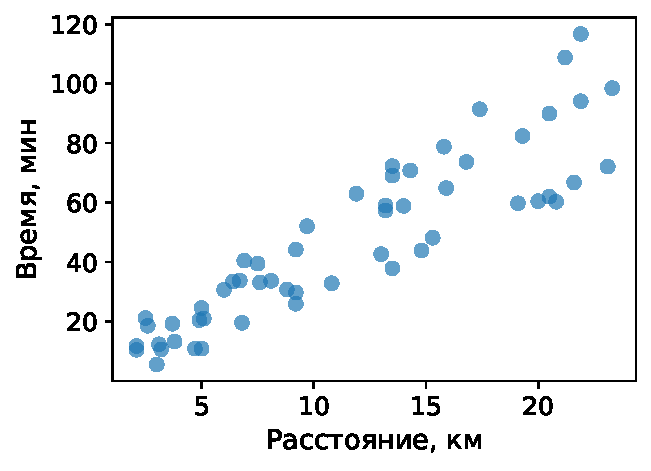
\includegraphics[width=\linewidth,height=0.59\textheight,keepaspectratio]{img/trips-mpl.pdf}
\end{column}
\end{columns}
\medskip
\small На рисунке 55 точек. Часть разброса связана с разной скоростью велосипедов: одного расстояния недостаточно, чтобы точно предсказать время.
\end{frame}
\section{Seaborn: связываем график с таблицей}
\begin{frame}{Seaborn: связываем график с таблицей}
Seaborn — библиотека поверх Matplotlib, которая упрощает распространённые графики анализа данных. Ей можно передать всю таблицу и назвать столбцы для x, y и цвета. Она сама найдёт категории, назначит цвета и создаст легенду.
\medskip

Сначала построим ту же диаграмму рассеяния. Затем добавим информацию о типе велосипеда. Подписи через plt продолжат работать: основой рисунка остаётся Matplotlib. Переменная ax и здесь не обязательна.
\end{frame}
% example:sns-scatter
\begin{frame}[fragile]{Тот же график через Seaborn}
\begin{columns}[c,onlytextwidth]
\begin{column}{0.49\textwidth}
\begin{lstlisting}
import seaborn as sns

sns.scatterplot(data=trips,
    x="distance_km", y="minutes")
plt.xlabel("Расстояние, км")
plt.ylabel("Время, мин")
plt.show()
\end{lstlisting}
\end{column}
\begin{column}{0.49\textwidth}
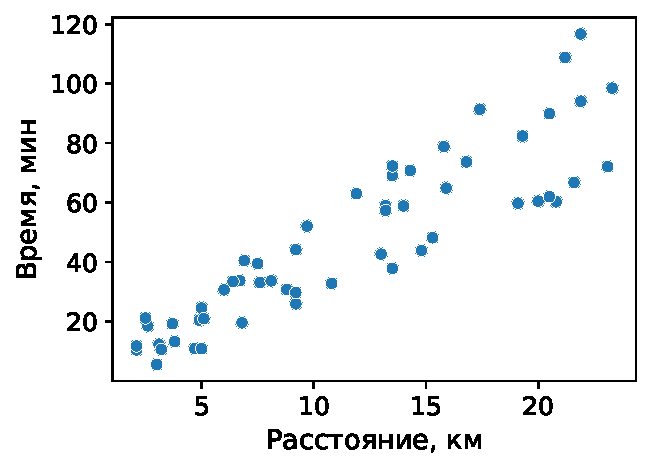
\includegraphics[width=\linewidth,height=0.59\textheight,keepaspectratio]{img/sns-scatter.pdf}
\end{column}
\end{columns}
\medskip
\small Координаты совпадают с предыдущим примером. Seaborn не добавляет новые поездки и не усредняет данные в scatterplot.
\end{frame}
% example:sns-hue
\begin{frame}[fragile]{Цвет показывает тип велосипеда}
\begin{columns}[c,onlytextwidth]
\begin{column}{0.49\textwidth}
\begin{lstlisting}
sns.scatterplot(data=trips,
    x="distance_km", y="minutes",
    hue="bike")
plt.xlabel("Расстояние, км")
plt.ylabel("Время, мин")
plt.legend(title="Велосипед", fontsize=8)
plt.show()
\end{lstlisting}
\end{column}
\begin{column}{0.49\textwidth}
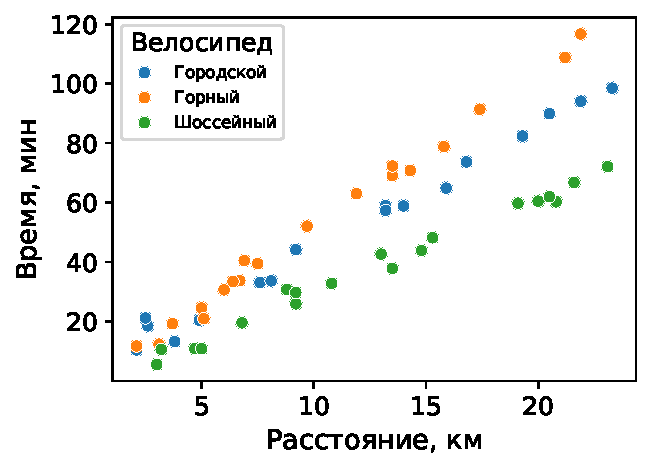
\includegraphics[width=\linewidth,height=0.59\textheight,keepaspectratio]{img/sns-hue.pdf}
\end{column}
\end{columns}
\medskip
\small hue="bike" задаёт цвет по типу велосипеда и создаёт легенду. Разные скорости здесь заложены в генераторе: это учебная модель, а не реальное измерение преимуществ велосипеда.
\end{frame}
% example:sns-strip
\begin{frame}[fragile]{Посмотрим на отдельные поездки в категориях}
\begin{columns}[c,onlytextwidth]
\begin{column}{0.49\textwidth}
\begin{lstlisting}
np.random.seed(1514)
sns.stripplot(data=trips,
    x="bike", y="minutes", jitter=True)
plt.xlabel("Велосипед")
plt.ylabel("Время, мин")
plt.xticks(rotation=15)
plt.show()
\end{lstlisting}
\end{column}
\begin{column}{0.49\textwidth}
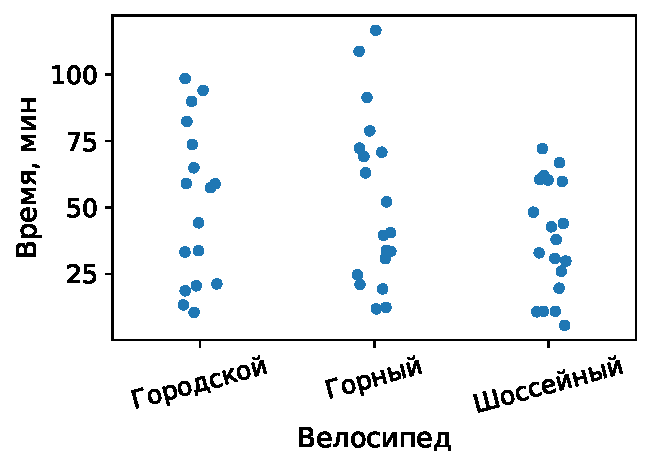
\includegraphics[width=\linewidth,height=0.59\textheight,keepaspectratio]{img/sns-strip.pdf}
\end{column}
\end{columns}
\medskip
\small seed фиксирует случайное горизонтальное смещение точек. Время внутри категории различается, ведь расстояния тоже разные. Сравнивать скорость только по этому рисунку было бы неправильно.
\end{frame}
\section{Встроенные графики pandas}
\begin{frame}{Встроенные графики pandas}
После Matplotlib и Seaborn познакомимся ещё с одной записью: Series.plot() и DataFrame.plot(). Эти методы позволяют построить распространённый график прямо из столбца или таблицы. По умолчанию pandas использует Matplotlib, поэтому знакомые подписи и сохранение через plt продолжают работать.
\medskip

kind задаёт тип: bar — столбцы, hist — гистограмма, scatter — точки, line — линии. Для Series подписи часто берутся из индекса, значения — из содержимого столбца. Для DataFrame мы явно укажем x и y. Создавать fig и ax для этих примеров не нужно.
\end{frame}
% example:pd-bar
\begin{frame}[fragile]{Series.plot: готовая выручка в виде столбцов}
\begin{columns}[c,onlytextwidth]
\begin{column}{0.49\textwidth}
\begin{lstlisting}
revenue_by_category.plot(
    kind="bar", rot=0
)
plt.xlabel("Категория")
plt.ylabel("Выручка, руб.")
plt.show()
\end{lstlisting}
\end{column}
\begin{column}{0.49\textwidth}
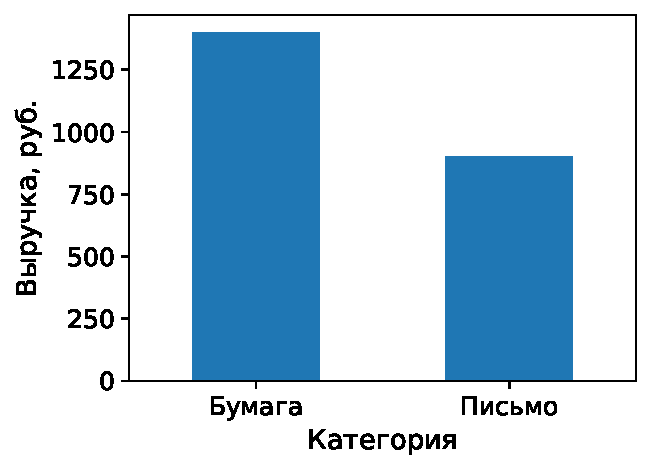
\includegraphics[width=\linewidth,height=0.59\textheight,keepaspectratio]{img/pd-bar.pdf}
\end{column}
\end{columns}
\medskip
\small Это тот же результат, что у plt.bar для сводки: 1400 и 900 рублей. rot=0 оставляет подписи горизонтальными; отдельный plt.figure не нужен.
\end{frame}
% example:pd-hist
\begin{frame}[fragile]{Гистограмма столбца из другого CSV}
\begin{columns}[c,onlytextwidth]
\begin{column}{0.49\textwidth}
\begin{lstlisting}
weather = pd.read_csv(
    DATA / "weather.csv"
)
weather["moscow"].plot(
    kind="hist",
    bins=[14, 16, 18, 20, 22, 24],
    edgecolor="white"
)
plt.xlabel("Температура, °C")
plt.ylabel("Число дней")
plt.show()
\end{lstlisting}
\end{column}
\begin{column}{0.49\textwidth}
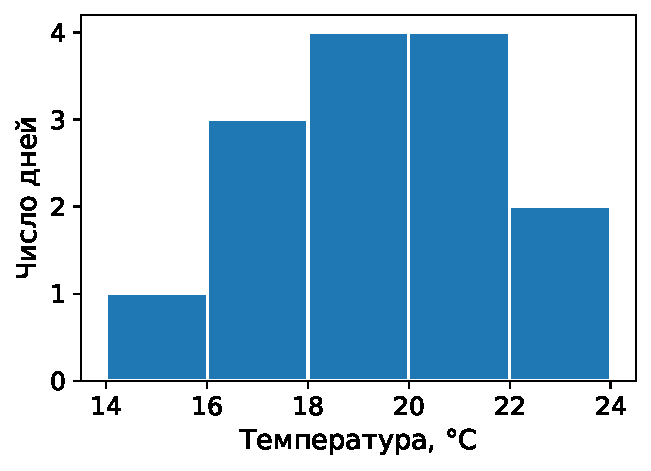
\includegraphics[width=\linewidth,height=0.59\textheight,keepaspectratio]{img/pd-hist.pdf}
\end{column}
\end{columns}
\medskip
\small Всего 14 наблюдений. Высота прямоугольника сообщает, сколько дней температура лежала в данном интервале, а не в какой день она наблюдалась.
\end{frame}
% example:pd-scatter
\begin{frame}[fragile]{DataFrame.plot: явно выбираем два столбца}
\begin{columns}[c,onlytextwidth]
\begin{column}{0.49\textwidth}
\begin{lstlisting}
trips.plot(kind="scatter",
    x="distance_km", y="minutes",
    alpha=0.7)
plt.xlabel("Расстояние, км")
plt.ylabel("Время, мин")
plt.show()
\end{lstlisting}
\end{column}
\begin{column}{0.49\textwidth}
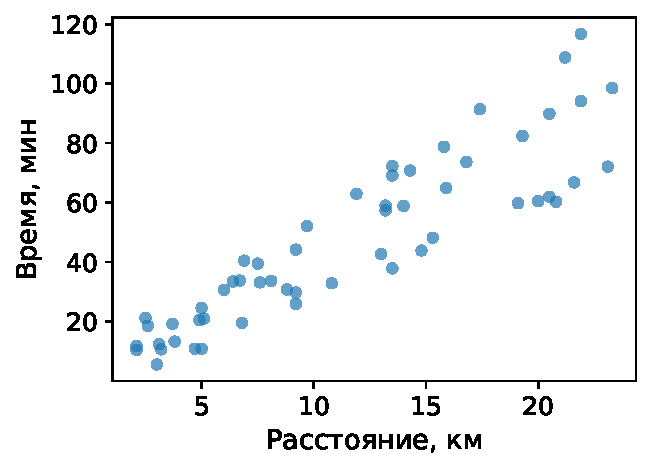
\includegraphics[width=\linewidth,height=0.59\textheight,keepaspectratio]{img/pd-scatter.pdf}
\end{column}
\end{columns}
\medskip
\small Снова те же 55 пар. Для быстрого графика этого достаточно; для удобного цвета по категориям можно вернуться к Seaborn и hue.
\end{frame}
% example:pd-lines
\begin{frame}[fragile]{Несколько линий из столбцов таблицы}
\begin{columns}[c,onlytextwidth]
\begin{column}{0.49\textwidth}
\begin{lstlisting}
weather.plot(x="day",
    y=["moscow", "kazan"], kind="line")
plt.xlabel("День")
plt.ylabel("Температура, °C")
plt.legend(["Москва", "Казань"])
plt.show()
\end{lstlisting}
\end{column}
\begin{column}{0.49\textwidth}
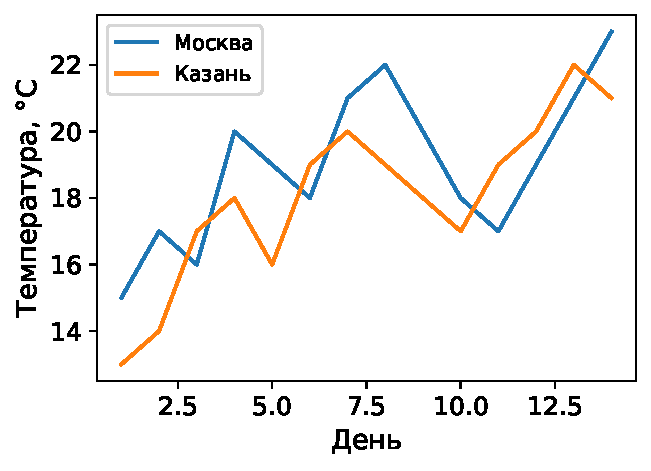
\includegraphics[width=\linewidth,height=0.59\textheight,keepaspectratio]{img/pd-lines.pdf}
\end{column}
\end{columns}
\medskip
\small Без kind по умолчанию тоже получились бы линии. Можно писать и сокращения: .plot.bar(), .plot.hist(), .plot.scatter(x=..., y=...).
\end{frame}
\section{Сохранение и самостоятельная работа}
\begin{frame}{Сохранение и самостоятельная работа}
Теперь мы умеем брать сведения из списка, таблицы или файла и выбирать график по вопросу. Линия показывает изменение по упорядоченному аргументу; точки — связь двух чисел; столбцы — значения категорий; гистограмма — распределение.
\medskip

pandas готовит данные и сводки, Seaborn помогает связывать визуальные свойства со столбцами, Matplotlib управляет самим рисунком. Способы можно сочетать: начать через pandas, а подписи и сохранение добавить через plt.
\end{frame}
% example:export-table
\begin{frame}[fragile]{Сохраним таблицу и прочитаем обратно}
\begin{columns}[c,onlytextwidth]
\begin{column}{0.49\textwidth}
\begin{lstlisting}
summary = revenue_by_category.reset_index(
    name="revenue"
)
summary.to_csv(
    OUTPUT / "sales_summary.csv",
    index=False)
pd.read_csv(OUTPUT / "sales_summary.csv")
\end{lstlisting}
\end{column}
\begin{column}{0.49\textwidth}
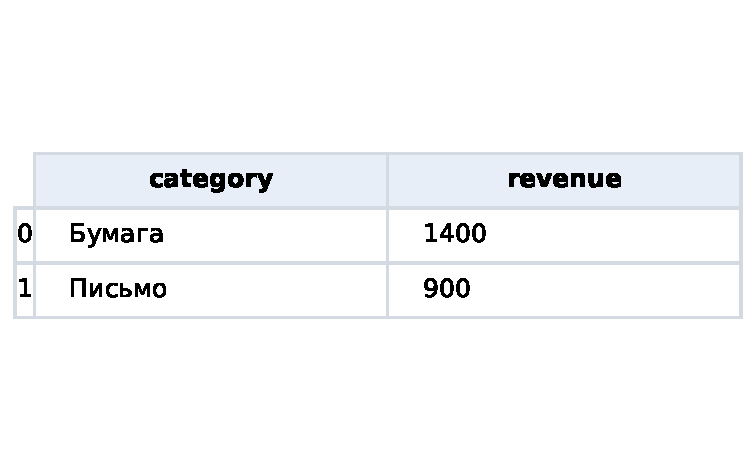
\includegraphics[width=\linewidth,height=0.59\textheight,keepaspectratio]{img/export-table.pdf}
\end{column}
\end{columns}
\medskip
\small Справа — результат обратного чтения сохранённого файла, а не вручную набранная копия. Папка OUTPUT настроена в начале ноутбука.
\end{frame}
% example:save-figure
\begin{frame}[fragile]{Сохранение рисунка не меняет его смысл}
\begin{columns}[c,onlytextwidth]
\begin{column}{0.49\textwidth}
\begin{lstlisting}
revenue_by_category.plot(
    kind="bar", rot=0)
plt.xlabel("Категория")
plt.ylabel("Выручка, руб.")
plt.savefig(OUTPUT / "sales.png", dpi=150,
            bbox_inches="tight")
plt.show()
\end{lstlisting}
\end{column}
\begin{column}{0.49\textwidth}
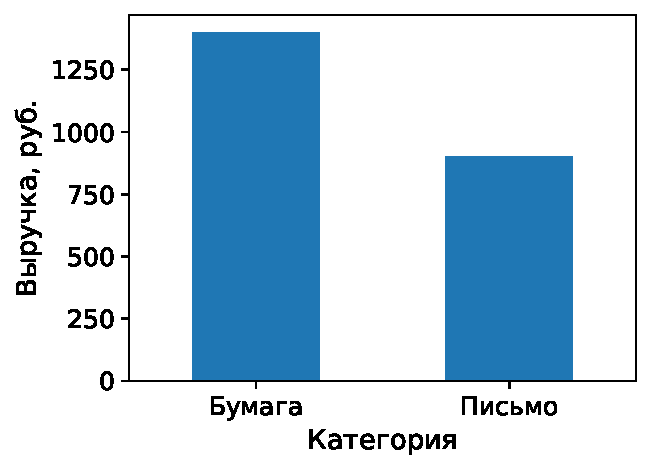
\includegraphics[width=\linewidth,height=0.59\textheight,keepaspectratio]{img/save-figure.pdf}
\end{column}
\end{columns}
\medskip
\small Справа тот же рисунок, который записан в sales.png. Перед публикацией проверьте подписи, единицы измерения и смысл каждой высоты.
\end{frame}
\section{Дополнительно: несколько областей рисунка}
\begin{frame}{Дополнительно: несколько областей рисунка}
Для одного рисунка достаточно разобранных команд plt. Если нужны две независимые области рядом, удобно получить явные переменные. fig обозначает весь рисунок, axes[0] и axes[1] — его области.
\medskip

Это дополнительный способ управления, а не обязательный шаг перед каждым графиком. Методы областей похожи на знакомые функции: axes[0].hist вместо plt.hist, set\_xlabel вместо xlabel.
\end{frame}
% example:two-axes
\begin{frame}[fragile]{Два вопроса на одном рисунке}
\begin{columns}[c,onlytextwidth]
\begin{column}{0.49\textwidth}
\begin{lstlisting}
fig, axes = plt.subplots(
    1, 2, figsize=(5.5, 3.3),
    layout="constrained")
axes[0].hist(trips["distance_km"], bins=5)
axes[0].set_xlabel("Км")
axes[0].set_ylabel("Число поездок")
axes[1].scatter(trips["distance_km"],
                trips["minutes"], s=12)
axes[1].set_xlabel("Км")
axes[1].set_ylabel("Минуты")
plt.show()
\end{lstlisting}
\end{column}
\begin{column}{0.49\textwidth}
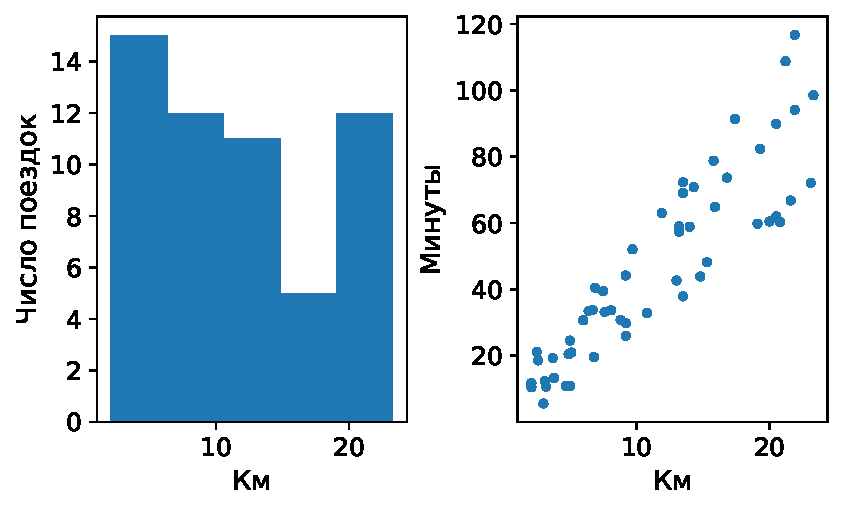
\includegraphics[width=\linewidth,height=0.59\textheight,keepaspectratio]{img/two-axes.pdf}
\end{column}
\end{columns}
\medskip
\small Здесь переменные областей действительно полезны: понятно, куда направлена каждая команда. В обязательном ДЗ этот интерфейс не требуется.
\end{frame}
\begin{frame}{Что сделать самостоятельно}
Домашнее задание находится в hw/homework.ipynb. Первые четыре задания — графики по спискам: погода, растения и поездки. Затем — небольшая таблица растений, чтение CSV о поездках, группировка, встроенные графики pandas и Seaborn.
\medskip
Для обязательной части не нужны fig и ax. Перед сдачей перезапустите ядро, выполните все ячейки и сохраните ноутбук с рисунками и пояснениями.
\medskip
\href{https://matplotlib.org/stable/}{Matplotlib} · \href{https://pandas.pydata.org/docs/}{pandas} · \href{https://seaborn.pydata.org/}{Seaborn}
\end{frame}
\end{document}
